\documentclass{standalone}
\usepackage{tikz}
\usetikzlibrary{patterns, positioning}


\begin{document}
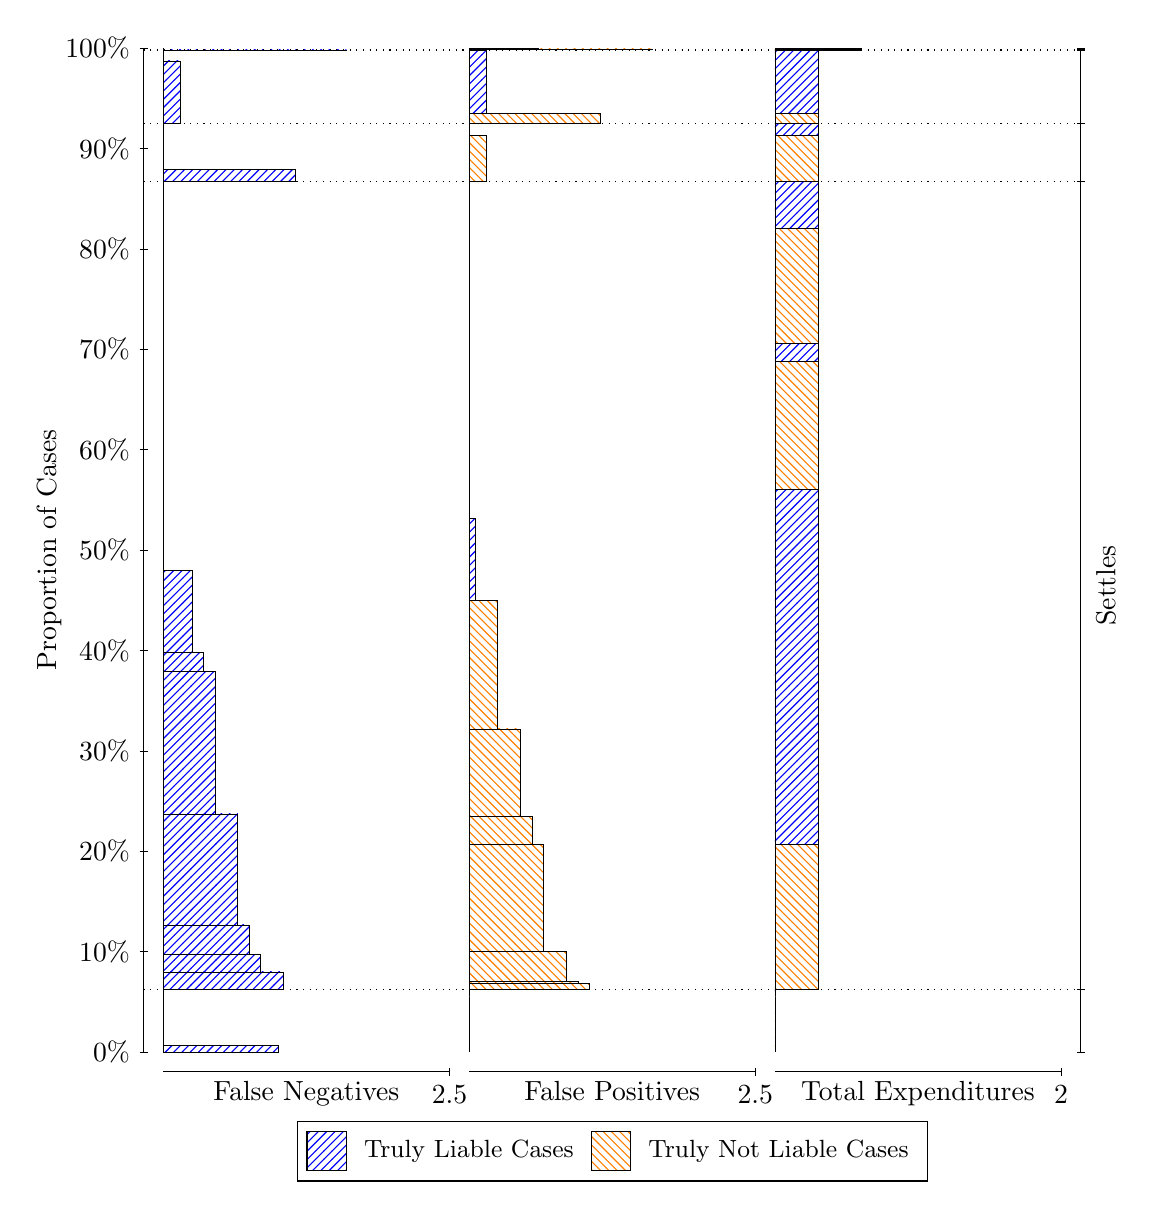
\begin{tikzpicture}
\draw[black, very thin] (1.5,1.75) -- (1.5,14.5);
\node[rotate=90, text=black, anchor=center] at (0.3, 8.125) {Proportion of Cases};
\draw[black, very thin] (1.45,1.75) -- (1.55,1.75);
\node[text=black, anchor=east] at (1.45, 1.75) {0\%};
\draw[black, very thin] (1.45,3.025) -- (1.55,3.025);
\node[text=black, anchor=east] at (1.45, 3.025) {10\%};
\draw[black, very thin] (1.45,4.3) -- (1.55,4.3);
\node[text=black, anchor=east] at (1.45, 4.3) {20\%};
\draw[black, very thin] (1.45,5.575) -- (1.55,5.575);
\node[text=black, anchor=east] at (1.45, 5.575) {30\%};
\draw[black, very thin] (1.45,6.85) -- (1.55,6.85);
\node[text=black, anchor=east] at (1.45, 6.85) {40\%};
\draw[black, very thin] (1.45,8.125) -- (1.55,8.125);
\node[text=black, anchor=east] at (1.45, 8.125) {50\%};
\draw[black, very thin] (1.45,9.4) -- (1.55,9.4);
\node[text=black, anchor=east] at (1.45, 9.4) {60\%};
\draw[black, very thin] (1.45,10.675) -- (1.55,10.675);
\node[text=black, anchor=east] at (1.45, 10.675) {70\%};
\draw[black, very thin] (1.45,11.95) -- (1.55,11.95);
\node[text=black, anchor=east] at (1.45, 11.95) {80\%};
\draw[black, very thin] (1.45,13.225) -- (1.55,13.225);
\node[text=black, anchor=east] at (1.45, 13.225) {90\%};
\draw[black, very thin] (1.45,14.5) -- (1.55,14.5);
\node[text=black, anchor=east] at (1.45, 14.5) {100\%};

\draw[black, very thin] (13.4,1.75) -- (13.4,14.5);
\draw[black, very thin] (13.35,1.75) -- (13.45,1.75);
\node[anchor=west] at (13.35, 1.75) {};
\draw[black, very thin] (13.35,2.5408) -- (13.45,2.5408);
\node[anchor=west] at (13.35, 2.5408) {};
\draw[black, very thin] (13.35,12.809) -- (13.45,12.809);
\node[anchor=west] at (13.35, 12.809) {};
\draw[black, very thin] (13.35,13.54) -- (13.45,13.54);
\node[anchor=west] at (13.35, 13.54) {};
\draw[black, very thin] (13.35,14.472) -- (13.45,14.472);
\node[anchor=west] at (13.35, 14.472) {};
\draw[black, very thin] (13.35,14.484) -- (13.45,14.484);
\node[anchor=west] at (13.35, 14.484) {};
\draw[black, very thin] (13.35,14.5) -- (13.45,14.5);
\node[anchor=west] at (13.35, 14.5) {};

\draw[black, very thin, pattern color=blue, pattern=north east lines] (1.75,1.75) rectangle (3.2033,1.8332);
\draw[black, very thin, pattern color=orange, pattern=north west lines] (1.75,1.8332) rectangle (1.75,2.5408);
\draw[black, very thin, pattern color=blue, pattern=north east lines] (1.75,2.5408) rectangle (3.276,2.7673);
\draw[black, very thin, pattern color=blue, pattern=north east lines] (1.75,2.7673) rectangle (2.9853,2.9871);
\draw[black, very thin, pattern color=blue, pattern=north east lines] (1.75,2.9871) rectangle (2.84,3.3634);
\draw[black, very thin, pattern color=blue, pattern=north east lines] (1.75,3.3634) rectangle (2.6947,4.7746);
\draw[black, very thin, pattern color=blue, pattern=north east lines] (1.75,4.7746) rectangle (2.404,6.5801);
\draw[black, very thin, pattern color=blue, pattern=north east lines] (1.75,6.5801) rectangle (2.2587,6.8275);
\draw[black, very thin, pattern color=blue, pattern=north east lines] (1.75,6.8275) rectangle (2.1133,7.8669);
\draw[black, very thin, pattern color=orange, pattern=north west lines] (1.75,7.8669) rectangle (1.75,12.809);
\draw[black, very thin, pattern color=blue, pattern=north east lines] (1.75,12.809) rectangle (3.4213,12.961);
\draw[black, very thin, pattern color=orange, pattern=north west lines] (1.75,12.961) rectangle (1.75,13.54);
\draw[black, very thin, pattern color=blue, pattern=north east lines] (1.75,13.54) rectangle (1.968,14.338);
\draw[black, very thin, pattern color=orange, pattern=north west lines] (1.75,14.338) rectangle (1.75,14.472);
\draw[black, very thin, pattern color=blue, pattern=north east lines] (1.75,14.472) rectangle (4.0753,14.477);
\draw[black, very thin, pattern color=orange, pattern=north west lines] (1.75,14.477) rectangle (1.75,14.484);
\draw[black, very thin, pattern color=orange, pattern=north west lines] (1.75,14.484) rectangle (1.75,14.489);
\draw[black, very thin, pattern color=blue, pattern=north east lines] (1.75,14.489) rectangle (1.75,14.5);
\draw[black, very thin, pattern color=orange, pattern=north west lines] (5.6333,1.75) rectangle (5.6333,2.4576);
\draw[black, very thin, pattern color=blue, pattern=north east lines] (5.6333,2.4576) rectangle (5.6333,2.5408);
\draw[black, very thin, pattern color=orange, pattern=north west lines] (5.6333,2.5408) rectangle (7.1593,2.6216);
\draw[black, very thin, pattern color=orange, pattern=north west lines] (5.6333,2.6216) rectangle (7.014,2.6457);
\draw[black, very thin, pattern color=orange, pattern=north west lines] (5.6333,2.6457) rectangle (6.8687,3.0285);
\draw[black, very thin, pattern color=orange, pattern=north west lines] (5.6333,3.0285) rectangle (6.578,4.3879);
\draw[black, very thin, pattern color=orange, pattern=north west lines] (5.6333,4.3879) rectangle (6.4327,4.7404);
\draw[black, very thin, pattern color=orange, pattern=north west lines] (5.6333,4.7404) rectangle (6.2873,5.8532);
\draw[black, very thin, pattern color=orange, pattern=north west lines] (5.6333,5.8532) rectangle (5.9967,7.4832);
\draw[black, very thin, pattern color=blue, pattern=north east lines] (5.6333,7.4832) rectangle (5.706,8.5227);
\draw[black, very thin, pattern color=blue, pattern=north east lines] (5.6333,8.5227) rectangle (5.6333,12.809);
\draw[black, very thin, pattern color=orange, pattern=north west lines] (5.6333,12.809) rectangle (5.8513,13.389);
\draw[black, very thin, pattern color=blue, pattern=north east lines] (5.6333,13.389) rectangle (5.6333,13.54);
\draw[black, very thin, pattern color=orange, pattern=north west lines] (5.6333,13.54) rectangle (7.3047,13.674);
\draw[black, very thin, pattern color=blue, pattern=north east lines] (5.6333,13.674) rectangle (5.8513,14.472);
\draw[black, very thin, pattern color=orange, pattern=north west lines] (5.6333,14.472) rectangle (5.6333,14.479);
\draw[black, very thin, pattern color=blue, pattern=north east lines] (5.6333,14.479) rectangle (5.6333,14.484);
\draw[black, very thin, pattern color=orange, pattern=north west lines] (5.6333,14.484) rectangle (7.9587,14.489);
\draw[black, very thin, pattern color=blue, pattern=north east lines] (5.6333,14.489) rectangle (6.5053,14.5);
\draw[black, very thin, pattern color=orange, pattern=north west lines] (9.5167,1.75) rectangle (9.5167,2.4576);
\draw[black, very thin, pattern color=blue, pattern=north east lines] (9.5167,2.4576) rectangle (9.5167,2.5408);
\draw[black, very thin, pattern color=orange, pattern=north west lines] (9.5167,2.5408) rectangle (10.062,4.3879);
\draw[black, very thin, pattern color=blue, pattern=north east lines] (9.5167,4.3879) rectangle (10.062,8.8914);
\draw[black, very thin, pattern color=orange, pattern=north west lines] (9.5167,8.8914) rectangle (10.062,10.521);
\draw[black, very thin, pattern color=blue, pattern=north east lines] (9.5167,10.521) rectangle (10.062,10.748);
\draw[black, very thin, pattern color=orange, pattern=north west lines] (9.5167,10.748) rectangle (10.062,12.213);
\draw[black, very thin, pattern color=blue, pattern=north east lines] (9.5167,12.213) rectangle (10.062,12.809);
\draw[black, very thin, pattern color=orange, pattern=north west lines] (9.5167,12.809) rectangle (10.062,13.389);
\draw[black, very thin, pattern color=blue, pattern=north east lines] (9.5167,13.389) rectangle (10.062,13.54);
\draw[black, very thin, pattern color=orange, pattern=north west lines] (9.5167,13.54) rectangle (10.062,13.674);
\draw[black, very thin, pattern color=blue, pattern=north east lines] (9.5167,13.674) rectangle (10.062,14.472);
\draw[black, very thin, pattern color=orange, pattern=north west lines] (9.5167,14.472) rectangle (10.607,14.479);
\draw[black, very thin, pattern color=blue, pattern=north east lines] (9.5167,14.479) rectangle (10.607,14.484);
\draw[black, very thin, pattern color=orange, pattern=north west lines] (9.5167,14.484) rectangle (10.607,14.489);
\draw[black, very thin, pattern color=blue, pattern=north east lines] (9.5167,14.489) rectangle (10.607,14.5);
\draw[black, dotted] (1.5,2.5408) -- (13.4,2.5408);
\draw[black, dotted] (1.5,12.809) -- (13.4,12.809);
\draw[black, dotted] (1.5,13.54) -- (13.4,13.54);
\draw[black, dotted] (1.5,14.472) -- (13.4,14.472);
\draw[black, dotted] (1.5,14.484) -- (13.4,14.484);
\draw[black, very thin] (1.75,1.5) -- (5.3833,1.5);
\node[text=black, anchor=north] at (3.5667, 1.5) {False Negatives};
\draw[black, very thin] (5.3833,1.45) -- (5.3833,1.55);
\node[text=black, anchor=north] at (5.3833, 1.45) {2.5};

\draw[black, very thin] (5.6333,1.5) -- (9.2667,1.5);
\node[text=black, anchor=north] at (7.45, 1.5) {False Positives};
\draw[black, very thin] (9.2667,1.45) -- (9.2667,1.55);
\node[text=black, anchor=north] at (9.2667, 1.45) {2.5};

\draw[black, very thin] (9.5167,1.5) -- (13.15,1.5);
\node[text=black, anchor=north] at (11.333, 1.5) {Total Expenditures};
\draw[black, very thin] (13.15,1.45) -- (13.15,1.55);
\node[text=black, anchor=north] at (13.15, 1.45) {2};


\node[text=black, centered, rotate=90] at (13.72, 7.6751) {Settles};





\draw (7.449999999999999,1.5) node[draw=none] (baseCoordinate) {};
\begin{scope}[align=center]
        \matrix[scale=0.5, draw=black, below=0.5cm of baseCoordinate, nodes={draw}, column sep=0.1cm]{
            \node[rectangle, draw, minimum width=0.5cm, minimum height=0.5cm, pattern color=blue, pattern=north east lines] {}; &
            \node[draw=none, font=\small, text=black] (B) {Truly Liable Cases}; &
            \node[rectangle, draw, minimum width=0.5cm, minimum height=0.5cm, pattern color=orange, pattern=north west lines] {}; &
            \node[draw=none, font=\small, text=black] (B) {Truly Not Liable Cases}; \\
            };
\end{scope}

\end{tikzpicture}
\end{document}